%!TEX root = ../dissertation.tex

\begin{savequote}[75mm]
Another inspiring quote for this chapter
\qauthor{Another author maybe}
\end{savequote}


\chapter[An early health technology assessment in the Netherlands]{Cost-Effectiveness Analysis of CT-Based Finite Element Modelling for Osteoporosis Screening in secondary fracture prevention: An early health technology assessment in the Netherlands}

\lettrine[lines=3]{\textcolor{SchoolColor}{{\bf O}}}{
{\bf bjective:} To conduct cost-utility analyses for Computed} Tomography To Strength (CT2S), a novel osteoporosis screening service, compared to dual-energy X-ray absorptiometry (DXA), Treat all without screening, and No Screening methods for Dutch postmenopausal women referred to fracture liaison service (FLS). CT2S employs CT scans to generate femur models and simulate sideways fall scenarios for bone strength assessment.

{\bf Methods:} Adopted early health technology assessment (HTA) to evaluate CT2S as a novel osteoporosis screening tool for secondary fracture prevention. We constructed a two-dimensional simulation model considering four strategies (No Screening, Treat all without screening, DXA, CT2S) together with screening intervals (5 years, 2 years), treatments (oral alendronate, zoledronic acid) and discount rate scenarios, among Dutch women in three age groups (60s, 70s, and 80s). Strategy comparisons were based on cost-effectiveness ratios (ICERs), considering an ICER below \texteuro 20,000 per QALY gained as cost-effective in the Netherlands.

{\bf Results:} Under the base case scenario, CT2S vs. DXA had estimated ICERs of \texteuro 41,200 and \texteuro 14,083 per QALY gained for 60s and 70s age groups, respectively. For the 80s age group, CT2S was more effective and less costly than DXA. Changing treatment from weekly oral alendronate to annual zoledronic acid substantially decreased CT2S vs. DXA ICERs across all age groups. Setting the screening interval to 2 years increased CT2S vs. DXA ICERs to \texteuro 100,333, \texteuro 55,571, and \texteuro 15,750 per QALY gained for the 60s, 70s, and 80s age groups, respectively. In all simulated populations and scenarios, CT2S was cost-effective (in some cases dominant) compared with Treat all strategy and cost-saving (more effective and less costly) compared to No Screening.

{\bf Conclusion:} CT2S was estimated to be potentially cost-effective in the 70s and 80s age groups considering the willingness-to-pay (WTP) threshold of the Netherlands. This early HTA suggests CT2S as a potential novel osteoporosis screening tool for secondary fracture prevention. 

\section{Highlights}
\begin{enumerate}
\item For post-menopausal Dutch women who have been referred to FLS, direct access to CT2S may be cost-effective compared to DXA for age groups 70s and 80s, when considering the ICER threshold of the Netherlands. This study positions CT2S as a potential novel osteoporosis screening tool for secondary fracture prevention in the clinical setting.
\item A shorter screening interval of two years increases the effectiveness of both screening strategies, but the ICER of CT2S compared to DXA also increased substantially which made CT2S no longer cost-effective for the 70s age group, but it remains cost-effective for the age group in their 80s.
\item Annual zoledronic acid treatment with better adherence may contribute to lower cost-effectiveness ratio when comparing CT2S to DXA screening and Treat all strategies for all age groups.
\end{enumerate}

\section{Introduction}

In the last decade, specialised fracture and osteoporosis clinics called fracture liaison service (FLS), run by nurse practitioners and supervised by physicians, have been introduced in several countries including the Netherlands \cite{4-1}. Typically, FLS employ dual-energy x-ray absorptiometry (DXA) screening for the persons with previous fracture history to measure the areal bone mineral density (aBMD) and then offer treatment advice, if necessary, to the referring practitioner \cite{4-1}. This radiological exam directly gives a measure of the bone mineral content, which is compared with epidemiological data in order to evaluate its deviation from the average healthy population. However, the predictive performance of DXA in terms of fracture risk prediction is not perfect \cite{4-2,4-3,4-4}, depending on the characteristics of the individual patient. For this reason, various authors have proposed an alternative measurement technique, called Biomechanical Computed Tomography analysis (BCT), also known as a digital twin, using a low-dose CT scan and a patient-specific computer-based biophysics model to predict the fracture force of the femur \cite{4-4,4-5,4-6}. Computed Tomography To Strength (CT2S) is a particular implementation of the BCT, developed in collaboration between the University of Sheffield (UOS) and the University of Bologna (UNIBO) \cite{4-3,4-6,4-7}. 

 CT2S is run as an online service (https://ct2s.insigneo.org/ct2s/) hosted at the University of Sheffield. The user (usually clinician) would make a job request via the website. The user then uploads anonymised patient CT scans through the website’s secure portal. The CT scans are downloaded by the CT2S operator. The femur shape is segmented in 3D and meshed using finite elements. The local material property of the femur is estimated based on the CT attenuation. This fully personalised model of the femur is then used to simulate various sideways fall scenarios including all feasible ranges of loading directions to determine the failure load of the bone (i.e. bone strength) and the weakest orientation. This information is then used to calculate the Absolute Risk of Fracture at present, or time 0 (ARF0), which is the ratio between the number of falls (that led to fracture) over the total number of falls. The results are then summarised in a simple PDF file, which is sent back to the user who requested the job \cite{4-8}.

Evaluation of the CT2S approach showed better discrimination between fractured and non-fractured groups in a pair-matched elderly cohort of 98 women, who are prone to osteoporosis. The area under the receiver operating characteristic curve (AUC) was 0.85 using CT2S compared with 0.75 using the aBMD-DXA as the predictor \cite{4-3,4-6,4-7}. This study was conducted in a single National Health Service (NHS) centre at Sheffield in the United Kingdom. Similar results have also been shown in studies conducted in other countries \cite{4-9}, using cohorts of different age, race and sex. It is worth mentioning that other groups have used BCT to also analyse vertebral fracture \cite{4-9}.  However, such analysis has not been done using CT2S. Nevertheless, the question remains as to whether the higher costs associated with measuring the CT2S biomarker would be expected to translate into meaningful health benefits and whether those benefits would be expected to be cost-effective in osteoporosis screening in the Netherlands.

According to the Health Insurance Act (Zorgverzekeringswet), all residents of the Netherlands are legally obliged to take out standard health insurance \cite{4-10}. The cost of examinations and medications prescribed by the general practitioner or medical specialist is covered by the standard health insurance (e.g. DXA screening) \cite{4-11}. Each year, the government updates the national healthcare scheme and the insurance companies are mandated to incorporate changes within their offered benefits. Health policy decision makers would be interested in acknowledging whether the novel osteoporosis screening tools are potentially cost-effective relative to DXA for particular populations in order to consider further development, investments, and reimbursement policies. 

Early health technology assessment (HTA) is a methodology employed to evaluate the potential value and feasibility of emerging innovations at their early stages \cite{4-12}. Therefore, early HTA is necessary for providing the initial insight by revealing the cost and health quality outcome of different osteoporosis screening strategies. In this study, we adopted early HTA to assess the potential value of CT2S to be used as a novel osteoporosis screening tool. We used a two-dimensional simulation to estimate data on which a cost-utility analysis (CUA) was conducted for four strategies: CT2S, the standard of care represented by aBMD (hereafter referred to as `DXA') \cite{4-13}, treat all patients without screening and no screening in postmenopausal women referred for assessment to the FLS.

\section{Methods}
\subsection{Study Perspective}

The following cost-effectiveness analysis was conducted from a healthcare system perspective, as it considered the costs and consequences incurred by the healthcare system.

\subsection{Screening Scenarios and Strategies}

The following scenarios were simulated: three age groups (60s, 70s and 80 years), two screening intervals (5 years as the base case and 2 years in scenario analysis), two types of treatment (weekly oral alendronate as the base case and once-yearly intravenous infusion of zoledronic acid in scenario analysis) and two discount rates (4.0\% and 1.5\% for costs and effectiveness as the base case according to the Dutch guideline for economic evaluations in healthcare \cite{4-14} and 3\% rate for benefits as well as costs in scenario analysis). Each scenario consists of a combination of age groups, screening intervals, treatments and discount rates, with four strategies: CT2S screening, DXA screening, Treat all and No Screening, (Fig. \ref{fig:4-1}).

\begin{figure}[!h]
\centering
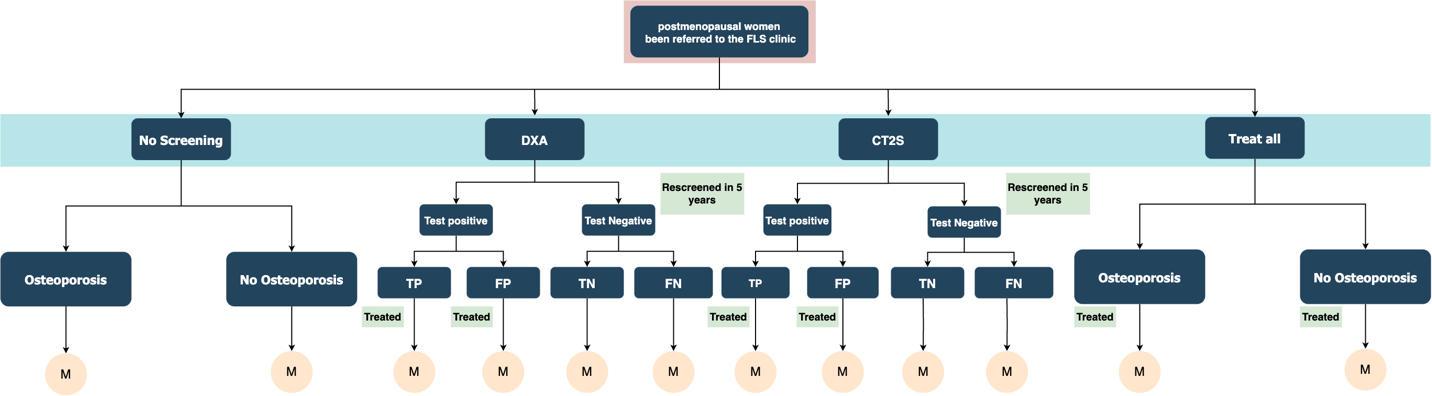
\includegraphics[width=1.0\textwidth]{4-1.png}
\caption{Diagram of screening model, TP = True Positive, FP = False Positive, TN = True Positive, FN = False Negative, M = Markov Chain.}
\label{fig:4-1}
\end{figure}

\subsection{Screening Interval}

In the literature, a variety of osteoporosis screening intervals have been suggested. An Australian clinical guideline for osteoporosis prevention and treatment suggests that follow-up screening should not be scheduled fewer than 2 years apart \cite{4-15}. A U.S. study shows that repeating BMD measurement after 8 years adds little marginal value in terms of predicting fractures beyond the initial testing \cite{4-16}. Another study from the University of Missouri-Columbia suggests that the rescreening interval should be 5 years for moderate osteopenia and 1 year for advanced osteopenia \cite{4-17}. There is no clear guideline whether the DXA scan should be performed only once or regularly in FLS.  However, the FLS model from a UK study indicates that FLS advises primary care clinicians to arrange follow up DXA monitoring after completion of 5 years of treatment \cite{4-18}. In addition, a longitudinal cohort study by Van Gompel et al. \cite{4-19} showed approximately 40\% of low-risk women and 60\% of high-risk or osteoporotic women were re-screened within 5 years. 

Women who received drug treatment after their initial DXA scan had a higher likelihood of undergoing short-interval repeat DXA scans \cite{4-19}. The frequency and type of follow-up screening for patients in FLS programs may vary depending on individual patient factors, and should be determined by a healthcare provider in consultation with the patient. In this study, the recommended procedures in the literature were followed and rescreening was simulated for all patients within the FLS, using a 5-year interval as a base case, and a 2-year interval as an alternate case.

\subsection{Screening Test Characteristics}

The receiver operating characteristic (ROC) curves for DXA and CT2S were obtained from the Sheffield cohort (98 subjects, 49 osteoporotic hip fractures and 49 controls) \cite{4-6}. Detailed descriptions of the CT2S pipeline methods and results on the Sheffield cohort can be found in previous studies \cite{4-3,4-6,4-7}. A brief description is provided here.

The Sheffield cohort is a retrospective cohort of 98 postmenopausal women, divided equally into two groups: a fracture group and a control group. The fracture group (n=49) consisted of women who had been diagnosed with low energy trauma fractures in the proximal femur (mean age 75 years). The control group (n=49) consisted of women who were pair-matched for age, height and weight. All patients received a DXA scan (Hologic Discovery scanner, Hologic Inc, Bedford, MA, USA) and a bilateral proximal femur CT scan (LightSpeed 64 VCT, GE Medical Systems, Milwaukee, WI, USA).

From the individual CT scans, the proximal femur of each patient was segmented by a trained mechanical engineer using ITK-Snap 2.0.0 (University of Pennsylvania). The segmented bone was fitted with 10-node tetrahedral finite elements using an averaged mesh size of 3 mm (ANSYS software). Element-based material property was estimated from the CT attenuation using Bonemat v3.0 \cite{4-20,4-21}. External load was applied to the personal-specific femur model in a range of possible sideways fall directions in ANSYS. The predicted maximum strain in the model was used to calculate bone strength for each individual. Subject-specific fall dynamics and hip impact mechanics were then incorporated into the model via ARF0 to obtain the final classification of fracture status and ROC curve.

To ensure a fair comparison, we chose biomarker thresholds were chosen to maximise the overall accuracy for both screening strategies (T score = $-1.41$ for DXA and ARF0 = 37.4\% for CT2S). These sensitivities and specificities were used to determine the true positive, false positive true negative and false negative probabilities in the simulation model (Table \ref{tab:4-1}). A percentile bootstrap method was used to construct 95\% confidence intervals (CI) for the sensitivity and specificity values \cite{4-22}. The stratification accuracy of DXA and CT2S in identifying osteoporotic hip fractures has been used as the approximation of the osteoporosis screening accuracy. In the screening arm, the model assumed that individuals identified as osteoporotic (true or false positives) would be treated with alendronate or zoledronic acid. We also modelled rescreening after a fracture \cite{4-23}.

\newpage
\begin{center}
\centering
\setlength{\tabcolsep}{0.8mm}{
\begin{longtable}{m{5.3cm}lll}
\caption{Key input parameters in the model}
\label{tab:4-1}\\
\toprule
\multirow{2}*{{\bf Parameter}} & {\bf Mean [95\% CI or} & \multirow{2}*{{\bf Distribution}} & \multirow{2}*{{\bf Source}}\\
 & {\bf estimates thereof]} & & \\
\midrule
\multicolumn{4}{l}{{\bf Screening performance of identifying osteoporosis}}\\
\midrule
DXA (T score = $-$1.41) sensitivity & 0.66 [0.524, 0.796] & Beta & Calculation $^{\mathrm{a}}$\\
DXA (T score = $-$1.41) specificity & 0.57 [0.426, 0.711] & Beta & Calculation $^{\mathrm{a}}$\\
CT2S (Threshold 37.4\%) sensitivity & 0.82 [0.753, 0.918] & Beta & \cite{4-6}\\
CT2S (Threshold 37.4\%) specificity & 0.78 [0.634, 0.865] & Beta & \cite{4-6}\\
\midrule
\multicolumn{4}{l}{{\bf Persistence of alendronate}}\\
\midrule
First year after treatment onset & 0.69 [0.552, 0.828] $^{\mathrm{b}}$ & Beta & \cite{4-38}\\
Second year after treatment onset & 0.563 [0.450, 0.676] $^{\mathrm{b}}$ & Beta & Calculation $^{\mathrm{c}}$\\
Third year after treatment onset & 0.436 [0.349, 0.523] $^{\mathrm{b}}$ & Beta & Calculation $^{\mathrm{c}}$\\
Fourth year after treatment onset & 0.309 [0.247, 0.371] $^{\mathrm{b}}$ & Beta & Calculation $^{\mathrm{c}}$\\
Fifth year after treatment onset & 0.182 [0.146, 0.218] $^{\mathrm{b}}$ & Beta & \cite{4-39}\\
\midrule
\multicolumn{4}{l}{{\bf Persistence of  zoledronic acid }}\\
\midrule
First year after treatment onset & 1.00 & Beta & \cite{4-41}\\
Second year after treatment onset & 0.73 [0.584, 0.876] & Beta & \cite{4-41}\\
Third year after treatment onset & 0.54 [0.432, 0.648] & Beta & \cite{4-41}\\
Fourth year after treatment onset & 0.40 [0.320, 0.480] & Beta & \cite{4-41}\\
Fifth year after treatment onset & 0.26 [0.213, 0.320] & Beta & Calculation $^{\mathrm{c}}$\\
Sixth year after treatment onset & 0.13 [0.107, 0.160] & Beta & Calculation $^{\mathrm{c}}$\\
\midrule
\multicolumn{4}{l}{{\bf RR of osteoporotic fracture with alendronate treatment}}\\
\midrule
Hip & 0.47 [0.26, 0.79] & Log normal & \cite{4-32}\\
Vertebral & 0.55 [0.36, 0.82] & Log normal & \cite{4-32}\\
Wrist & 0.70 [0.49, 0.98] & Log normal & \cite{4-32}\\
\midrule
\multicolumn{4}{l}{{\bf RR of osteoporotic fracture with zoledronic acid treatment}}\\
\midrule
Hip & 0.50 [0.34, 0.73] & Log normal & \cite{4-31}\\
Vertebral & 0.35 [0.20, 0.64] & Log normal & \cite{4-31}\\
Wrist & 0.75 [0.64, 0.87] & Log normal & \cite{4-33}\\
\midrule
\multicolumn{4}{l}{{\bf Osteoporosis prevalence}}\\
\midrule
50-54 years & 0.063 & Beta $^{\mathrm{d}}$ & \cite{4-43}\\
55-59 years & 0.096 & Beta $^{\mathrm{d}}$ & \cite{4-43}\\
60-64 years & 0.143 & Beta $^{\mathrm{d}}$ & \cite{4-43}\\
65-69 years & 0.202 & Beta $^{\mathrm{d}}$ & \cite{4-43}\\
70-74 years & 0.279 & Beta $^{\mathrm{d}}$ & \cite{4-43}\\
75-79 years & 0.375 & Beta $^{\mathrm{d}}$ & \cite{4-43}\\
80+years & 0.472 & Beta $^{\mathrm{d}}$ & \cite{4-43}\\
\midrule
\multicolumn{4}{l}{{\bf Osteoporosis prevalence in FLS Netherlands}}\\
\midrule
60s & 0.257 & Beta $^{\mathrm{d}}$ & \cite{4-44}\\
70s & 0.407 & Beta $^{\mathrm{d}}$ & Calculation $^{\mathrm{e}}$\\
80s & 0.552 & Beta $^{\mathrm{d}}$ & Calculation $^{\mathrm{e}}$\\
\midrule
{\bf Annual fracture incidence rate} & Appendix & Beta $^{\mathrm{d}}$ & \cite{4-47}\\
\midrule
\multicolumn{4}{l}{{\bf RR of subsequent fracture following a prior fracture}}\\
\midrule
Hip & 2.9 [2.0, 4.3] & Log normal & \cite{4-50}\\
Vertebral & 2.52 [1.99, 3.19] & Log normal & \cite{4-51}\\
Wrist & 1.69 [1.35, 2.12] & Log normal & \cite{4-51}\\
\midrule
{\bf RR of any subsequent fracture with prior fracture} & 1.86 [1.75, 1.98] & Log normal & \cite{4-49}\\
\midrule
\multicolumn{4}{l}{{\bf Osteoporosis attribution probabilities for hip fractures}}\\
%\bottomrule
%\end{longtable}}\vspace{-2.5em}
%\end{center}
%\begin{center}
%\centering
%\setlength{\tabcolsep}{0.8mm}{
%\begin{longtable}{llll}
%\caption{Key input parameters in the model}
%\label{tab:4-1}\\
%\toprule
\midrule
50-64 years & 0.8 [0.25, 0.80] & Beta & \cite{4-48}\\
65-84 years & 0.9 [0.80, 0.95] & Beta & \cite{4-48}\\
85+years & 0.95 [0.90, 1.0] & Beta & \cite{4-48}\\
\midrule
\multicolumn{4}{l}{{\bf Osteoporosis attribution probabilities for vertebral fractures}}\\
\midrule
50-64 years & 0.8 [0.50, 0.85] & Beta & \cite{4-48}\\
65-84 years & 0.9 [0.70, 0.95] & Beta & \cite{4-48}\\
85+years & 0.95 [0.80, 1.0] & Beta & \cite{4-48}\\
\midrule
\multicolumn{4}{l}{{\bf Osteoporosis attribution probabilities for wrist fractures}}\\
\midrule
50-64 years & 0.7 [0.10, 0.70] & Beta & \cite{4-48}\\
65-84 years & 0.7 [0.50 - 0.80] & Beta & \cite{4-48}\\
85+years & 0.8 [0.70 - 0.95] & Beta & \cite{4-48}\\
\midrule
\multicolumn{4}{l}{{\bf Probability of nursing home residency after hip fractures}}\\
\midrule
50-74 years & 0.06 [0.048, 0.072] $^{\mathrm{b}}$ & Beta & \cite{4-68}\\
75-79 years & 0.11 [0.088, 0.132] $^{\mathrm{b}}$ & Beta & \cite{4-68}\\
80+years & 0.65 [0.52, 0.78] $^{\mathrm{b}}$ & Beta & \cite{4-69}\\
\midrule
\multicolumn{4}{l}{{\bf Annual mortality rate}}\\
\midrule
60-64 years & 0.0062 & Beta $^{\mathrm{d}}$ & \cite{4-53}\\
65-69 years & 0.0094 & Beta $^{\mathrm{d}}$ & \cite{4-53}\\
70-74 years & 0.0151 & Beta $^{\mathrm{d}}$ & \cite{4-53}\\
75-79 years & 0.0255 & Beta $^{\mathrm{d}}$ & \cite{4-53}\\
80-85 years & 0.0489 & Beta $^{\mathrm{d}}$ & \cite{4-53}\\
85+years & 0.1439 & Beta $^{\mathrm{d}}$ & \cite{4-53}\\
\midrule
{\bf RR of mortality risk with osteoporosis} & 1.19 [1.04, 1.36] & Log normal & \cite{4-54}\\
\midrule
\multicolumn{4}{l}{{\bf RR of mortality risk with fracture}}\\
\midrule
Hip, first year & 2.87 [2.52, 3.27] & Log normal & \cite{4-55}\\
Hip, subsequent years & 1.78 [1.33, 2.39] & Log normal & \cite{4-55}\\
Vertebral, first year & 2.87 [2.52, 3.27] & Log normal & \cite{4-55}\\
Vertebral, subsequent years & 1.78 [1.33, 2.39] & Log normal & \cite{4-55}\\
Wrist & 1.43 [1.07, 1.92] & Log normal & \cite{4-59}\\
Excess mortality attributable to fracture & 0.25 & Beta $^{\mathrm{d}}$ & \cite{4-60,4-61}\\
\midrule
\multicolumn{4}{l}{{\bf Cost (\texteuro)}}\\
\midrule
\multicolumn{4}{l}{{\bf Average direct costs of the first year after fractures}}\\
\midrule
Hip fracture & 21476.78 $^{\mathrm{f}}$ & Gamma $^{\mathrm{d}}$ & \cite{4-63}\\
Vertebral fracture & 2740.15 $^{\mathrm{f}}$ & Gamma $^{\mathrm{d}}$ & \cite{4-64}\\
Wrist fracture & 1572.61 $^{\mathrm{f}}$ & Gamma $^{\mathrm{d}}$ & \cite{4-65}\\
\midrule
Annual medication (Alendronate) cost & 22.33 $^{\mathrm{f}}$ & Gamma $^{\mathrm{d}}$ & \cite{4-67}\\
DXA screening cost & 96.74 $^{\mathrm{f}}$ & Gamma $^{\mathrm{d}}$ & \cite{4-64}\\
CT2S screening cost & 274.29 & Gamma $^{\mathrm{d}}$ & Calculation $^{\mathrm{g}}$\\
Annual nursing home cost & 63549.45 $^{\mathrm{f}}$ & Gamma $^{\mathrm{d}}$ & \cite{4-70}\\
\midrule
\multicolumn{4}{l}{{\bf Health utility}}\\
\midrule
\multicolumn{4}{l}{{\bf Health utility general population}}\\
\midrule
45-54 years & 0.874 & Beta $^{\mathrm{d}}$ & \cite{4-72}\\
55-64 years & 0.869 & Beta $^{\mathrm{d}}$ & \cite{4-72}\\
65-74 years & 0.863 & Beta $^{\mathrm{d}}$ & \cite{4-72}\\
75+years & 0.798 & Beta $^{\mathrm{d}}$ & \cite{4-72}\\
\midrule
{\bf Health utility nursing home after hip fracture} & 0.40 [0.34, 0.46)] & Beta & \cite{4-74}\\
\midrule
\multicolumn{4}{l}{{\bf Health utility multiplier after fracture}}\\ 
\midrule
Hip, first year & 0.55 [0.53, 0.57] & Beta & \cite{4-73}\\
Hip, second year & 0.84 [0.82, 0.86] & Beta & \cite{4-73}\\
Hip, third and subsequent year & 0.86 [0.84, 0.89] & Beta & \cite{4-73}\\
Vertebral, first year & 0.68 [0.65, 0.70] & Beta & \cite{4-73}\\
Vertebral, second year & 0.84 [0.81, 0.88] & Beta & \cite{4-73}\\
Vertebral, third and subsequent year & 0.85 [0.82, 0.87] & Beta & \cite{4-73}\\
Wrist, first year & 0.83 [0.82, 0.84] & Beta & \cite{4-73}\\
Wrist, second year & 0.98 [0.97, 0.99] & Beta & \cite{4-73}\\
Wrist, third and subsequent year & 0.99 [0.97, 1.00] & Beta & \cite{4-73}\\
\midrule
\multicolumn{4}{l}{{\bf Annual discount rate \%}}\\
\midrule
Effectiveness & 1.50\% & - & \cite{4-14}\\
Cost & 4\% & - & \cite{4-14}\\
\bottomrule
\end{longtable}}
\begin{tablenotes}
\footnotesize
\item[a]$^{\mathrm{a}}$ Sensitivity and specificity for DXA are from the results for the Sheffield cohort reported above
\item[b]$^{\mathrm{b}}$ The value was varied by $\pm$20\% to create CI
\item[c]$^{\mathrm{c}}$ The percentage of patient stay on treatment of alendronate was calculated based on the first and fifth year data declines in a linear manner, same apply to oabtaining fifth and sixth year persistence data for zoledronic acid
\item[d]$^{\mathrm{d}}$ Standard deviation assumed to be 20\% of the mean
\item[e]$^{\mathrm{e}}$ The increment in the osteoporosis prevalence of general population was used to generate the moderate estimation of the osteoporosis prevalence for the 60s and 80s age groups within FLS
\item[f]$^{\mathrm{f}}$ Cost values were adjusted for the inflation rate in the Netherlands to year 2021
\item[g]$^{\mathrm{g}}$ The detailed calculation of CT2S service cost can be seen in the supplemental Appendix, Table \ref{tab:4-3}
\end{tablenotes}
\vspace{-2.5em}
\end{center}

\newpage
\subsection{Study Population}

This study was focused on the Dutch postmenopausal women (from 60 years old) who have been referred to the FLS with a recent clinical fracture.

\subsection{Structure of the Individual-level Model}

We employed a discrete-time, discrete-state, individual-level (microsimulation) model to simulate osteoporosis disease trajectories in order to estimate lifetime costs and quality-adjusted life years (QALYs) for each simulated individual under the various screening scenarios and strategies. The model considered 9 discrete health states: no osteoporosis, osteoporosis without experiencing any new fracture in our simulation, 3 main types of fractures (Hip, Vertebral and Wrist), the corresponding post fracture state and, finally, death (Fig. \ref{fig:4-2}). The model counted time from referral to a FLS until either death or age 100 years in discrete, one-year time steps (cycles). According to the Dutch guideline for economic evaluations in healthcare, annual discount rates of 4.0\% and 1.5\% have been used for costs and effectiveness, respectively \cite{4-14}. The model was constructed in TreeAge Pro 2021 R1 (TreeAge Pro Inc., Williamston, MA, USA).

\begin{figure}[!h]
\centering
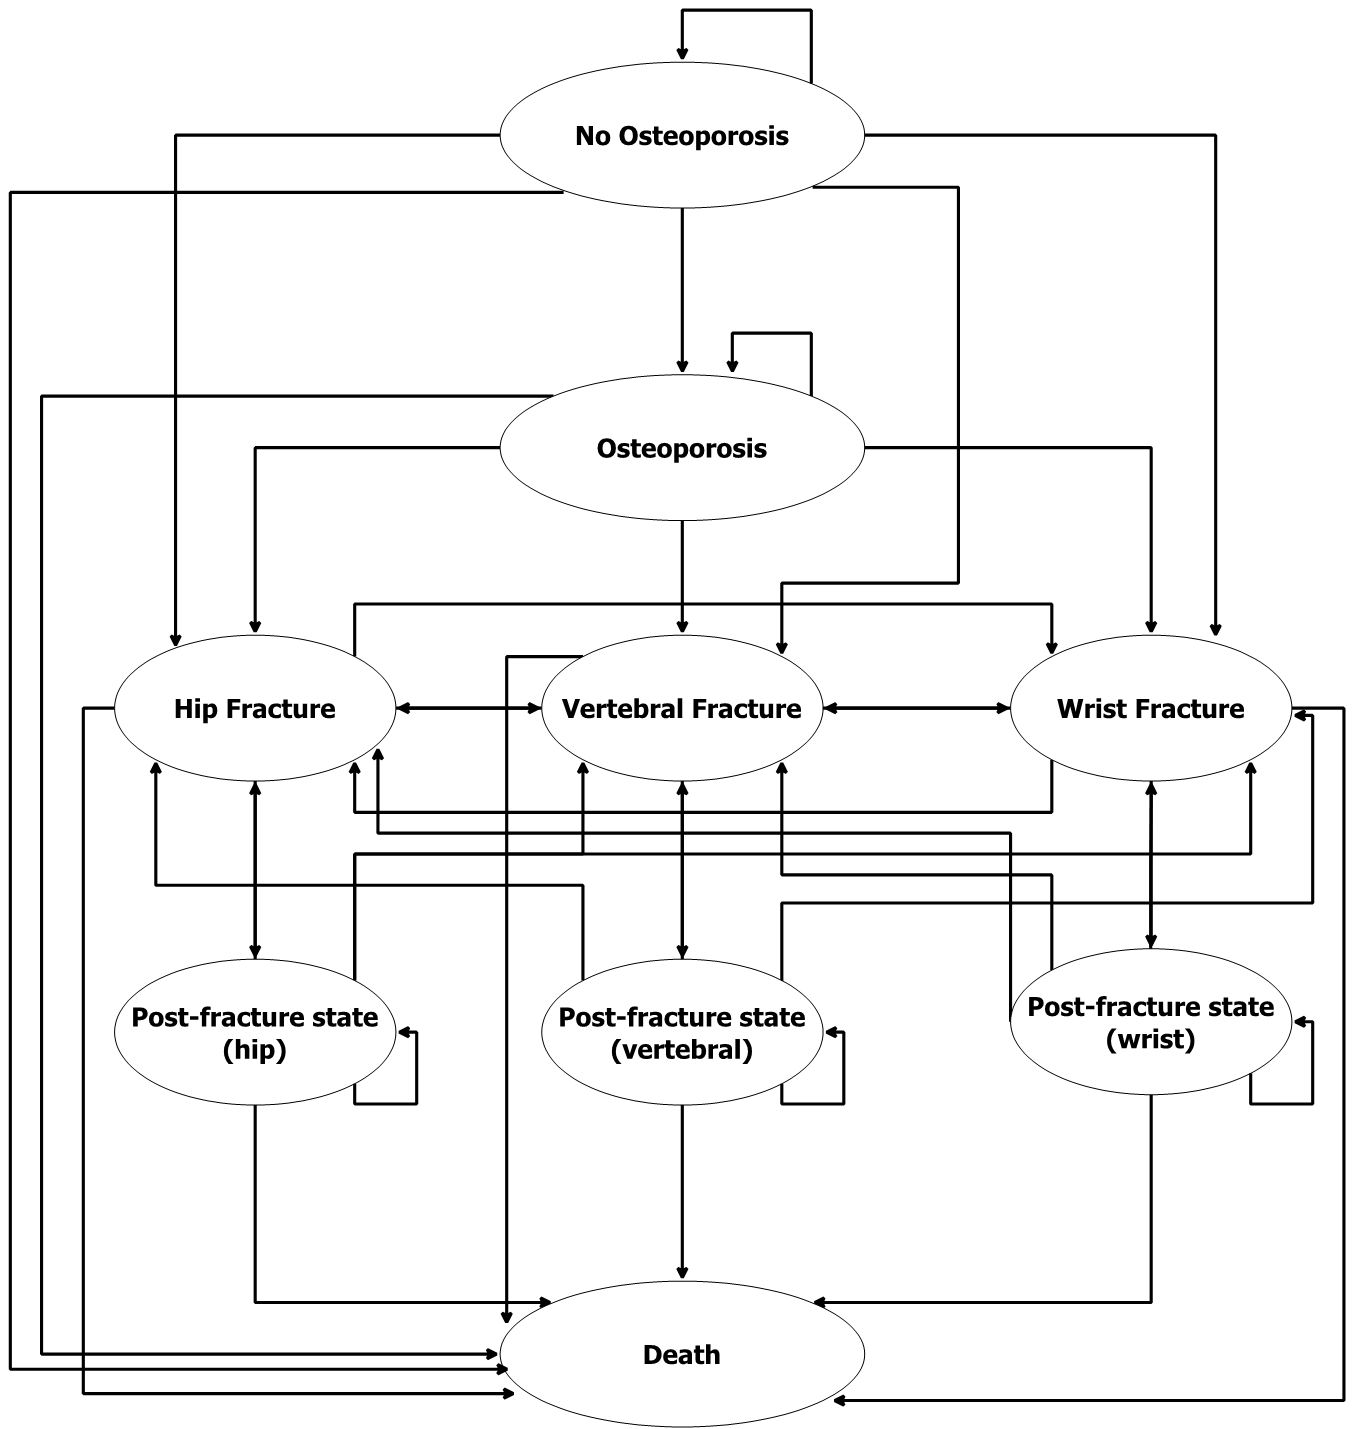
\includegraphics[width=0.8\textwidth]{4-2.png}
\caption{Structure of the Microsimulation Model.}
\label{fig:4-2}
\end{figure}

\subsection{Validation of the Individual-level Model}

The internal and external validation for the model were conducted based on guidelines from ISPOR \cite{4-24}. For internal validation, validation output generated from the model was used to compare with real, observed values from among the data used for creating the model. The prevalence of osteoporosis at different age groups were compared to assess the degree to which the model reproduced the observed data. For external validation, simulated validation output were compared with observed data from sources that were not used in the creation of the model: life expectancy and lifetime probability of fracture in women older than 50 and 80 years. The performed Goodness-of-fit analysis was performed by fitting a linear relationship between modelled and observed data. Model validity was assessed via the squared linear correlation coefficient (R$^2$). These analyses were performed using SPSS@ Statistics Version 25. Detailed validation approaches are elaborated upon in the Appendix (Sections Interval Validation and External Validation).

\subsection{Two-dimensional Simulation}

We employed a two-dimensional simulation \cite{4-25}. The two dimensions were defined in terms of parameter-level iterations and individual-level iterations. The parameter-level iterations captured input parameter uncertainty for parameters that were relevant for groups of persons while the individual-level iterations (microsimulations) captured patient-level stochasticity. For each scenario consisting of a combination of starting age, screening interval and CT2S cost, 10,000 parameter-level iterations were ran. For each parameter-level iteration, model input parameters were sampled from distributions. With each set of input parameters, 1000 iterations of the individual-level model (microsimulations) were simulated as described above. Each sampled individual then entered the microsimulation model four times, once for each of the strategies. Lifetime costs and QALYs for each strategy were then averaged across individual-level iterations, and grand averages were computed as averages of the individual-level averages across parameter-level iterations. Distributions of the model outputs - average lifetime costs and QALYs among parameter-level iterations provided an estimate of the combined uncertainty related to input parameter uncertainty and patient stochasticity. Despite the lack of reported confidence intervals or standard deviations for the health utility, osteoporosis prevalence, mortality rate, and annual fracture rate for the Dutch general population, we incorporated these values into our parameter-level sampling by estimating beta distributions. The standard deviation was estimated to be 20\% of the mean (Table \ref{tab:4-1}).  Moreover, the screening interval and discount rates were considered to be fixed values.

\subsection{Cost-Utility Analysis}

Using the simulated data, we performed CUAs. For each starting age, screening interval, treatment and discount rates scenario, the grand averages for the four strategies (CT2S, DXA, Treat all and No Screening) were recorded. Incremental cost-effectiveness ratios (ICERs) were calculated as the difference in lifetime costs divided by the difference in QALYs between pairs of strategies. A strategy was considered cost-effective if the Incremental Cost-Effectiveness Ratio (ICER) was below the lower bound ICER threshold set in the Netherlands (\texteuro 20,000/QALY gained) \cite{4-26}. If a strategy had lower estimated lifetime cost yet higher QALYs than its comparator, it was considered to dominate the comparator.

To assess the uncertainty in the CUAs, the net monetary benefit (NMB) was calculated for each parameter-level iteration and each strategy as $\lambda^* \mathrm{QAL} \mathrm{Y}_{\mathrm{ij}}-\mathrm{C}_{\mathrm{ij}}$ where `$\lambda$' is the willingness-to-pay (WTP) threshold expressed as the average cost of generating one additional quality-adjusted life year in the Netherlands, `i' is the index of the parameter-level iteration, `j' is the index of the strategy (0 for No Screening, 1 for DXA, 2 for CT2S and 3 for Treat all). QAL $\mathrm{Y}_{\mathrm{ij}}$ and $\mathrm{C}_{\mathrm{ij}}$ represent the QALYs and average lifetime cost estimated for the ith iteration of the jth strategy, respectively. In order to illustrate combined parameter-level and person-level uncertainty, we constructed cost-effectiveness acceptability curves (CEACs) where the value of $\lambda$ was varied, and at each value, the proportions of parameter-level iterations for which each strategy had the highest NMB was determined. The cost-effectiveness acceptability frontier (CEAF) was also constructed for comparison.

\subsection{One-Way Sensitivity Analysis}

We performed deterministic one-way sensitivity analysis (DSAs) to study the impact changes of each input parameter on the simulation results when all other input parameters were sampled as per usual. Screening sensitivity and specificity, fracture cost, fracture risks, discount rates, treatment efficacy, medication cost, excess mortality, fracture disutilities, screening interval and screening cost were included in the one-way sensitivity analyses. In each DSA, most of the given parameter varied from 80 to 120\% of its base case value \cite{4-27}. In order to reflect more uncertainty of the CT2S test characteristics, we expanded the sensitivity analyses of the CT2S test characteristics (both sensitivity and specificity) by varying the value from 70\% to 130\%, and incorporating more finely-grained intervals (10\%). The discount rate of effectiveness and cost were varied from 0\% to 6\%. The screening interval varied from 3 to 7 years. The gradient in average lifetime cost and the QALYs across the range of values employed for the DSA for No Screening, DXA, CT2S and Treat all were estimated for each input parameter.

\subsection{Model Input Parameter Data}
\subsubsection{Medication and Efficacy}

The bisphosphonate alendronate is the most frequently prescribed medication for osteoporosis in the Netherlands \cite{4-28}, weekly oral alendronate has been adopted in our base case analysis, together with the combination of vitamin D, calcium and lifestyle recommendation \cite{4-29}. Once-yearly intravenous infusion of zoledronic acid has become a popular alternative to oral alendronate for treating osteoporosis in postmenopausal women. This treatment has better adherence and similar effectiveness in reducing the risks of different types of fractures \cite{4-30,4-31} . Therefore as part of our scenario analyses, annual zoledronic acid treatment was also considered. The relative risk (RR) of osteoporotic fracture with alendronate and zoledronic acid treatment are presented in Table \ref{tab:4-1} \cite{4-31,4-32,4-33}.

\subsubsection{Treatment Duration and Adherence}

Based on the NHS guidance in the UK, it may take 6 to 12 months for alendronate to be fully effective in terms of bone protection \cite{4-34}. Since the cycle length of our simulation was 1 year, we assumed no treatment efficacy if the treatment was discontinued within the first year. Several studies have recommended applying a `drug holiday' after 5 years of continuous alendronate treatment, which is in accordance with evidence to show that the residual effect of the alendronate will be sustained for up to 5 years \cite{4-35,4-36}. Therefore, we assumed that the maximum duration of continuous alendronate prescription was 5 years with a residual effect that declined linearly to 0 over a 5-year period after treatment was discontinued \cite{4-37}. Two studies of alendronate treatment in postmenopausal women with osteoporosis showed that 69\% of people remained on treatment after 1 year \cite{4-38} while 18.2\% received the full 5 years of treatment \cite{4-39}. We assumed the percentage of people staying on treatment declined in a linear manner and calculated the discontinuation rate of alendronate treatment from year 1 to 5.

A study of the effect of zoledronic acid treatment shows that there is no significant difference in treatment efficacy between the patients with 6 versus 9 years of treatment \cite{4-40}. Since the residual effect of zoledronic acid could be up to 3 years \cite{4-30}, we assumed that the maximum duration of continuous alendronate treatment was 6 years and the residual effect of zoledronic acid will be declined in linear manner to 0 over a 3-year period after treatment was discontinued. Only one study of zoledronic acid reported the yearly percentage of patient stay on treatment from year 1 to 4 \cite{4-41}. We made the assumption that the proportion of patients who remained on the treatment would decrease in a linear fashion for year 5 and 6. For both alendronate and zoledronic acid treatment, re-treatment was modelled to be provided if a fracture occurred or the rescreening result was positive. Treatment was also provided to woman who initially screened negative but subsequently screened positive.

\subsubsection{Osteoporosis Prevalence and Incidence}

Osteoporosis-related studies revealed that the prevalence of osteoporosis in the Netherlands is 1.9 per 1000 for men and 16.1 per 1000 for women and increases with age \cite{4-29,4-42}. However, specific osteoporosis prevalence data for elderly women across age groups were not available for the Dutch population. Therefore, data from a Swedish population study was employed \cite{4-43}. Since the current study is focused on Dutch postmenopausal women referred to the FLS, the Swedish data were supplemented with the reported osteoporosis prevalence of the people referred to the FLS in the Netherlands \cite{4-44}. Due to the fact that the osteoporosis prevalence of the 5 FLSs study were not reported by sex, the model's osteoporosis prevalence estimate (40.7\%) was obtained for women within the 70s age group from the FLS with the highest proportion of female persons (88.2\%), which also had an average age of 69 \cite{4-44}. Since data from the Netherlands FLS lacked detailed osteoporosis prevalence for the 60s and 80s age group for women, the increment in the osteoporosis prevalence of the general population was used and the osteoporosis prevalence were estimated to be 25.7\% and 55.2\% for each of the age groups, respectively (Table \ref{tab:4-1}). The incidence of osteoporosis based on the difference of osteoporosis prevalence plus the mortality rate for the specific age group was estimated \cite{4-45}. We considered the differences in the prevalence of osteoporosis as 5-year cumulative osteoporosis incidence to calculate the 1-year incidence rate and transition probability of developing osteoporosis \cite{4-46}. Detailed calculations of osteoporosis transition probability are elaborated upon in the Appendix (Section Transition Probability of Developing Osteoporosis).

\subsubsection{Fracture Rates}

The age-specific annual hip, vertebral and wrist fracture rates were obtained for general population from the Dutch-specific osteoporosis reports by the International Osteoporosis Foundation (IOF) \cite{4-47}. We calculated the annual osteoporotic fracture incidence rate using the annual incident rate of fracture for the general population times Melton's osteoporosis attributed rates \cite{4-48} and then divided by the prevalence of osteoporosis for that age band. Subsequently, the annual incidence rate was translated to transition probability using equation 2 shown in Appendix \cite{4-46}. Since all people in FLS had a previous history of fracture, the fracture rates for people experiencing `first fracture' in our simulation were adjusted by multiplying the relative risks (RRs) of any secondary fracture for people with a previous fracture history (1.86 according to Kanis's study) \cite{4-49}. Simulated people in our model could suffer more than one fracture and the risk of sustaining a subsequent fracture was therefore set higher than the initial fracture risk. The RRs of secondary hip, vertebral and wrist fractures were therefore obtained as 2.9, 2.52 and 1.69, respectively \cite{4-50,4-51}. The corresponding transition probabilities of fractures per cycle are calculated based on the annual fracture rates \cite{4-46}. Detailed age specific annual fracture rates and the calculations of the osteoporotic fracture probabilities are elaborated in the Appendix (Section Fracture rates for Dutch general population and osteoporotic fracture rates calculations).

\subsubsection{Mortality Rate}

Consistent with the previous economic evaluations of  secondary fracture prevention intervention \cite{4-52}, age-specific, general population mortality risks for Dutch women were derived from the Global Health Observatory data repository published by the World Health Organisation (WHO) as our baseline mortality rates \cite{4-53}. Mortality risk of osteoporotic individuals were higher than the general population (RR= 1.19), this value has been applied to the patients having osteoporosis but without experiencing `first fracture' in our simulation \cite{4-54}. The relative mortality risk of people with and without hip fractures within the general population is 2.87 and 1.78 for the first and subsequent years, respectively \cite{4-55}. Several studies have shown that the excess mortality rate after vertebral fracture is similar to those of hip fracture \cite{4-56,4-57,4-58}. Therefore in the model, the relative mortality risk after vertebral and hip fracture was assumed to be the same. Excess mortality rate after wrist fracture was estimated to be 1.43 \cite{4-59}. Since comorbidities could also be a contributing factor to excess mortality, the proportion of the excess mortality following fractures attributable to the fractures themselves was assumed to be 25\% \cite{4-60,4-61}, therefore, the excess mortality of hip, vertebral, and wrist fractures have been adjusted accordingly to avoid overcounting. Besides, consistent with the previous economic evaluations of osteoporosis intervention \cite{4-62}, the model considers only the additional mortality caused by hip or vertebral fractures in patients who have experienced both non-hip/non-vertebral fractures and hip/vertebral fractures. In the case of patients who have multiple hip or vertebral fractures, or both types of fractures, only one excess mortality value was included in the model.

\subsubsection{Costs}

The following cost items were considered in our model: direct cost of fractures, annual medication cost, screening cost and nursing home costs after hip fracture. In the first year post fracture, the direct costs associated with hip, vertebral and wrist fracture in the Netherlands were reported to be \texteuro 21,477, \texteuro 2,740 and \texteuro 1,573, respectively \cite{4-63,4-64,4-65}. A study revealed a substantial rise in the use of generic alendronate among the Dutch population since its availability in 2005, with up to 62\% of patients opting for this medication by 2011 \cite{4-66}. Furthermore, the Dutch health insurance companies tend to reimburse more affordable generic form of drug. Therefore, our study incorporated the annual cost of generic alendronate in the Netherlands \cite{4-67}. When a hip fracture occurred, patients either entered into a nursing home or the community for recovery and the corresponding transition probabilities have been applied \cite{4-68,4-69}. The annual cost of nursing home residence (\texteuro 63,549) was calculated using the subtraction of the total cost of a person with a hip fracture confined to a nursing home and the first-year direct cost of hip fracture \cite{4-70}. The DXA scan price in the Netherlands is \texteuro 96.74 \cite{4-64}. The cost of the CT2S screening was calculated with the following components: CT scan cost, computing cost, storage cost of raw data, licence cost and personnel cost. The average cost of CT2S screening was estimated to be \texteuro 274 (Table \ref{tab:4-3}, Appendix). All costs were adjusted for the inflation rate in the Netherlands to the 2022 value \cite{4-71}. We assumed everybody received sufficient calcium and vitamin D so the costs of supplements were not included in the model.


\begin{center}
\centering
%\setlength{\tabcolsep}{0.8mm}{
\begin{longtable}{lllll}
\caption{Lifetime healthcare costs, QALYs, averaged across simulation iterations and incremental cost-effectiveness ratio of CT2S compared with DXA, Treat all and No screening for the various age groups under the base case scenario: weekly oral alendronate treatment, screening interval = 5 years, discount rates are 4.0\% and 1.5\% for costs and effectiveness.}
\label{tab:4-2}\\
\toprule
 & {\bf CT2S} & {\bf DXA} & {\bf Treat all} & {\bf No screening}\\
\midrule
{\bf Women aged 60-70 y} &   &   &   &  \\
Cost & \texteuro  7,177 & \texteuro  6,765 & \texteuro  7,082 & \texteuro  7,694\\
QALY & 14.080 & 14.070 & 14.025 & 13.998\\
ICER &   & \texteuro  41,200 & \texteuro  1,727* & Cost-saving\\
{\bf Women aged 70 $-$80 y}  &   &   &  \\
Cost & \texteuro  9,768 & \texteuro  9,599 & \texteuro  10,216 & \texteuro  11,338\\
QALY & 9.491 & 9.479 & 9.449 & 9.403\\
ICER &   & \texteuro  14,083* & Dominant & Cost-saving\\
{\bf Women aged 80 $-$90 y}  &   &   &  \\
Cost & \texteuro  13,553 & \texteuro  13,712 & \texteuro  13,534 & \texteuro  16,520\\
QALY & 5.286 & 5.275 & 5.274 & 5.212\\
ICER &   & Dominant & \texteuro  1,583* & Cost-saving\\
\bottomrule
\end{longtable}%}
\begin{tablenotes}
\footnotesize
\item[a] Dominant = CT2S more QALYs, lower costs than DXA or Treat all. Cost-saving = CT2S more QALY and lower costs than No screening 
\item[b] *Using the lower bound of WTP threshold in the Netherlands (\texteuro 20,000), these values are considered cost-effective for CT2S compared against DXA or Treat All
\end{tablenotes}
%\vspace{-2.5em}
\end{center}


\begin{center}
\centering
\setlength{\tabcolsep}{0.8mm}{
\begin{longtable}{m{6cm}m{2cm}<{\centering}m{2.3cm}<{\centering}m{1.8cm}<{\centering}}
\caption{One-way sensitivity analyses on the incremental cost-effectiveness ratio of CT2S vs No screening, CT2S vs DXA, and CT2S vs Treat all for the 70s age group under the base case scenario: with weekly oral alendronate treatment and 5 years screening interval, discount rates 4.0\% and 1.5\% for costs and effectiveness.}
\label{tab:4-3}\\
\toprule
{\bf Parameters} & \multicolumn{3}{c}{{\bf ICER}} \\
\midrule
 & {\bf CT2S vs No screening} & {\bf CT2S vs DXA} & {\bf CT2S vs Treat all}\\
\midrule
{\bf Base case} & Cost-saving & 14,083 & Dominant\\
\midrule
0.8 times DXA screening cost & Cost-saving & 20,214 & Dominant\\
1.2 times DXA screening cost & Cost-saving & 15,524 & Dominant\\
0.8 times Annual nursing home cost & Cost-saving & 18,571 & Dominant\\
1.2 times Annual nursing home cost & Cost-saving & 12,476 & Dominant\\
0.8 times DXA screening sensitivity & Cost-saving & Dominant & Dominant\\
1.2 times DXA screening sensitivity & Cost-saving & 112,711 & Dominant\\
0.8 times DXA screening specificity & Cost-saving & 17,850 & Dominant\\
1.2 times DXA screening specificity & Cost-saving & 13,265 & Dominant\\
0.7 times CT2S screening sensitivity & Cost-saving & Dominated by DXA & 3,984\\
0.8 times CT2S screening sensitivity & Cost-saving & Dominated by DXA & Dominant\\
0.9 times CT2S screening sensitivity & Cost-saving & 24,751 & Dominant\\
1.1 times CT2S screening sensitivity & Cost-saving & 2,870 & Dominant\\
1.2 times CT2S screening sensitivity & Cost-saving & Dominant & Dominant\\
1.3 times CT2S screening sensitivity (sensitivity = 1\dag) & Cost-saving & Dominant & Dominant\\
0.7 times CT2S screening specificity & Cost-saving & 5,234 & Dominant\\
0.8 times CT2S screening specificity & Cost-saving & 8,937 & Dominant\\
0.9 times CT2S screening specificity & Cost-saving & 12,956 & Dominant\\
1.1 times CT2S screening specificity & Cost-saving & 15,173 & Dominant\\
1.2 times CT2S screening specificity & Cost-saving & 20,834 & Dominant\\
1.3 times CT2S screening specificity (specificity = 1\dag\dag) & Cost-saving & 32,123 & Dominant\\
screening interval = 3 & Cost-saving & 34,957 & Dominant\\
screening interval = 7 & Cost-saving & 4,680 & Dominant\\
0.8 times CT2S screening cost & Cost-saving & 2,222 & Dominant\\
1.2 times CT2S screening cost & Cost-saving & 28,825 & Dominant\\
discount rate = 0\% & Cost-saving & 4,586 & Dominant\\
discount rate = 6\% & Cost-saving & 30,077 & Dominant\\
0.8 times Excess mortality attributable to fracture & Cost-saving & 16,210 & Dominant\\
1.2 times Excess mortality attributable to fracture & Cost-saving & 13,071 & Dominant\\
0.8 times alendronate persistence & Cost-saving & 24,029 & Dominant\\
1.2 times alendronate persistence & Cost-saving & 10,712 & Dominant\\
0.8 times annual fracture rate general population & Cost-saving & 20,557 & Dominant\\
1.2 times annual fracture rate general population & Cot-saving & 7,214 & Dominant\\
0.8 times Fracture disutilities & Cost-saving & 24,968 & Dominant\\
1.2 times Fracture disutilities & Cost-saving & 10,578 & Dominant\\
0.8 times Fracture cost & Cost-saving & 17,931 & Dominant\\
1.2 times Fracture cost & Cost-saving & 13,117 & Dominant\\
0.8 times base case treatment efficacy & Cost-saving & 27,109 & Dominant\\
1.2 times base case treatment efficacy & Cost-saving & 7,436 & Dominant\\
0.8 times annual medication cost & Cost-saving & 14,224 & Dominant\\
1.2 times annual medication cost & Cost-saving & 13,927 & Dominant\\
\bottomrule
\end{longtable}}
\begin{tablenotes}
\footnotesize
\item[a] Dominant = CT2S more QALYs, lower costs than DXA or Treat all. Dominated by DXA =  CT2S lower QALYs, more costs than DXA.  Cost-saving = CT2S more QALY and lower costs than no screening
\item[b] \dag Note tht the absolute value of sensitivity has exceeded 1 when CT2S screening sensitivity was increased by 30\%
\item[c] \dag\dag Note tht the absolute value of specificity has exceeded 1 when CT2S screening specificity was increased by 30\%
\end{tablenotes}
%\vspace{-2.5em}
\end{center}

\subsubsection{Health-State Utility Values}

The health utilities values were obtained from a previous application of the EQ-5D multidimensional health index to a sample from the general population in the Netherlands, responses on the five domains of the index were mapped to utility values using the European VAS value set scoring algorithm \cite{4-72}. The baseline health-state utility values for patients with prior fractures were estimated by multiplying the health-state utility of the general population by 0.85, a health utility multiplier for subsequent years ($> 2$ years) after a prior vertebral fracture. This is consistent with the previous economic evaluations of fracture liaison services patients \cite{4-52}. Since fractures and post fracture recovery will be associated with a decline in quality-of-life, we applied a health utility multiplier of the subsequent years after fractures in our simulation \cite{4-73}. In addition, the health utility of 0.4 was used for those people entering nursing homes after a hip fracture \cite{4-74}.

\section{Results}
\subsection{Internal and External Validation Results}

For internal validation, the modelled and observed prevalence of osteoporosis were compared. The squared correlation coefficient (R2) was 0.998. For external validation, the R$^2$ was jointly calculated for life expectancy and fracture risk and the value was 0.988. The collective results are shown in Table \ref{tab:4-1} and Table \ref{tab:4-2} in the supplemental Appendix.

\subsection{Base Case Analysis}

Grand averages of lifetime costs and QALYs, as well as cost-utility analyses results are presented in Table \ref{tab:4-2}. In the base case analysis, the screening interval was set to 5 years, with discount rates of 4.0\% for costs and 1.5\% for effectiveness (according to the Dutch guideline for economic evaluations in healthcare). The treatment strategy involved weekly oral alendronate treatment. The ICERs of CT2S vs. DXA for the age groups of 60s and 70s were \texteuro 41,200 and \texteuro 14,083, respectively, per QALY gained. For the 80s age group, CT2S was dominant (an increase in QALYs at lower lifetime cost) compared with DXA screening. The ICERs of CT2S vs. Treat all strategy for the age groups of 60s and 80s were \texteuro 1,727 and \texteuro 1,583, respectively. For the 70s age group, CT2S was dominant compared with Treat all. In all simulated populations, CT2S was cost-saving (more effective and less costly)  compared to the No Screening scenario. According to the cost-effectiveness in practice published by the Dutch National Health Care Institute, the WTP threshold in the Netherlands varies from \texteuro 20,000 to \texteuro 80,000 \cite{4-26}. In this study, we conservatively used \texteuro 20,000 to evaluate the cost-effectiveness of the screening strategies across all populations and scenarios. The results indicated that ICER of CT2S vs. DXA for the 70s and 80s age groups is less than the lower bound ICER threshold (\texteuro 20,000) in the Netherlands. It is worth mentioning that the QALY outcomes of the Treat all strategy without screening are always lower than those with screening. Treatment adherence is considered in our model and the lifetime horizon simulation also simulates the progression of patients developing osteoporosis. Even though Treat all strategy treat all patients referred to the FLSs at the beginning, the rescreening process can identify those patients who developed osteoporosis after treatment discontinuation. The targeted treatment will impact the final outcomes of QALY and cost for each individual patient referred to the FLSs. However, we observed that the gap in QALY outcomes between the Treat all strategy and CT2S or DXA screening diminishes as the simulation group ages. This is largely due to the increase in osteoporosis prevalence in the older age group and shorter simulated lifetime.

\subsection{One-Way Sensitivity Analysis}

Table \ref{tab:4-3} reported the result of one-way sensitivity analysis in women in their 70s using the base case scenario: with the screening interval of 5 years, discount rates at 4.0\% and 1.5\% for costs and effectiveness with weekly oral alendronate treatment. In all the sensitivity analyses, CT2S was cost-saving compared with No Screening scenario. Furthermore, CT2S dominated Treat all strategy in most of the sensitivity analyses, except when CT2S sensitivity was at $-$30\%. In that case, the ICER of CT2S versus Treat all was \texteuro 3,984.  

When comparing CT2S with DXA, the CT2S sensitivity had a marked impact on the ICER outcome. When CT2S sensitivity increased by 10\%, the ICER of CT2S vs. DXA was \texteuro 2,870. When CT2S sensitivity increased by 20\% and 30\%, CT2S dominated DXA. On the contrary, when CT2S sensitivity decreased by 10\%, the ICER of CT2S vs. DXA was \texteuro 24,751. When CT2S sensitivity decreased by 20\% and 30\%, DXA dominated CT2S. This is expected as the sensitivity of CT2S decreases (by 20\% or more), its ability to identify osteoporosis patients reduces, making it less superior compared with DXA.  Similarly, When DXA sensitivity decreased by 20\%, the CT2S method became dominant compared with DXA. Conversely, when the sensitivity of DXA increased by 20\%, the ICER of CT2S vs. DXA increased to \texteuro 112,711.

The results were also strongly affected by other parameters such as screening interval and the cost of CT2S. The ICER of CT2S compared to DXA more than doubled when the screening interval was equal to 3 years. The ICER of CT2S vs. DXA decreased to \texteuro 2,222 when the CT2S cost decreased by 20\%. Moreover, the ICER of CT2S vs. DXA increased to \texteuro 27,109 if the medication efficacy decreased by 20\%. The decrease in medication persistence resulted in lower QALY and higher cost and changed the ICER of CT2S vs. DXA to \texteuro 24,029. Cost per QALY increased to \texteuro 30,077 when the discount rate increased to 6\% and decreased to \texteuro 4,586 when the discount rate decreased to 0\%, respectively. Additionally, when the specificity of CT2S varied from $-$30\% to $+$30\%, the ICER continued to increase. 

\subsection{Alternative Scenario Analyses}

As an extension to the base case scenario, we extended our analysis to also consider: (a) alternative discount rate (3\% rate for benefits as well as costs used in other countries), (b) alternative treatment of once-yearly intravenous infusion of zoledronic acid, and (c) alternative screening interval of 2 years in the scenario analyses. The results for these alternative scenarios were presented in Table \ref{tab:4-4}.

\begin{center}
\centering
%\setlength{\tabcolsep}{0.8mm}{
\begin{longtable}{lllll}
\caption{ICER of CT2S screening compared with DXA, Treat all and No Screening with three alternative scenarios: discount rate = 3\%, annual zoledronic acid treatment and 2-year screening interval scenarios. For each alternative scenario, the other parameters were kept the same as the base case scenario.}
\label{tab:4-4}\\
\toprule
 & {\bf CT2S} & {\bf DXA} & {\bf Treat all} & {\bf No screening}\\
\midrule
\multicolumn{4}{l}{{\bf (a) Discount rate = 3\%}}\\
\midrule
{\bf Women aged 60-70 y} &   &   &  &  \\
Cost & \texteuro  8,666 & \texteuro  8,235 & \texteuro  8,692 & \texteuro  9,459\\
QALY & 11.962 & 11.954 & 11.925 & 11.900\\
ICER &   & \texteuro  53,875 & Dominant & Cost-saving\\
{\bf Women aged 70 -80 y} &   &   &  &  \\
Cost & \texteuro  11,041 & \texteuro  10,888 & \texteuro  11,626 & \texteuro  12,894\\
QALY & 8.462 & 8.452 & 8.431 & 8.390\\
ICER &   & \texteuro  15,300* & Dominant & Cost-saving\\
{\bf Women aged 80 -90 y} &   &   &   &  \\
Cost & \texteuro  14,267 & \texteuro  14,448 & \texteuro  14,322 & \texteuro  17,431\\
QALY & 4.923 & 4.913 & 4.914 & 4.857\\
ICER &   & Dominant & Dominant & Cost-saving\\
\midrule
\multicolumn{4}{l}{{\bf (b) Annual zoledronic acid treatment}}\\
\midrule 
{\bf Women aged 60-70 y} &   &   &   &  \\
Cost & \texteuro  6,998 & \texteuro  6,626 & \texteuro  7,023 & \texteuro  7,674\\
QALY & 14.111 & 14.093 & 14.034 & 13.991\\
ICER &   & \texteuro  20,667 & Dominant & Cost-saving\\
{\bf Women aged 70 -80 y} &   &   &   &  \\
Cost & \texteuro  9,511 & \texteuro  9,397 & \texteuro  10,120 & \texteuro  11,340\\
QALY & 9.529 & 9.510 & 9.469 & 9.404\\
ICER &   & \texteuro  6,000* & Dominant & Cost-saving\\
{\bf Women aged 80 -90 y} &   &   &   &  \\
Cost & \texteuro  13,005 & \texteuro  13,269 & \texteuro  13,228 & \texteuro  16,484\\
QALY & 5.314 & 5.299 & 5.293 & 5.211\\
ICER &   & Dominant & Dominant & Cost-saving\\
\midrule
\multicolumn{4}{l}{{\bf (c) Screening interval = 2 years}}\\
\midrule
{\bf Women aged 60-70 y} &   &   &   &  \\
Cost & \texteuro  7,886 & \texteuro  6,682 & \texteuro  7,078 & \texteuro  7,694\\
QALY & 14.109 & 14.097 & 14.018 & 13.991\\
ICER &   & \texteuro  100,333 & \texteuro  8,879* & \texteuro  1,627*\\
{\bf Women aged 70 -80 y} &   &   &   &  \\
Cost & \texteuro  9,909 & \texteuro  9,131 & \texteuro  10,202 & \texteuro  11,325\\
QALY & 9.525 & 9.511 & 9.449 & 9.403\\
ICER &   & \texteuro  55,571 & Dominant & Cost-saving\\
{\bf Women aged 80 -90 y} &   &   &   &  \\
Cost & \texteuro  13,068 & \texteuro  12,879 & \texteuro  13,550 & \texteuro  16,527\\
QALY & 5.310 & 5.298 & 5.275 & 5.211\\
ICER &   & \texteuro  15,750* & Dominant & Cost-saving\\
\bottomrule
\end{longtable}%}
\begin{tablenotes}
\footnotesize
\item[a] Dominant = CT2S more QALYs, lower costs than DXA or Treat all. Cost-saving = CT2S more QALY and lower costs than no screening
\item[a] *Using the lower bound of WTP threshold in the Netherlands (\texteuro 20,00), these values are considered cost-effective for CT2S compared against DXA, Treat All or No screening  
\end{tablenotes}
%\vspace{-2.5em}
\end{center}

In the 3\% discount rate scenario (screening interval = 5 years, weekly oral alendronate treatment), the ICER of CT2S vs. DXA in the 60s age group was \texteuro 53,875, which exceeded the willingness-to-pay (WTP) threshold of the Netherlands (\texteuro 20,000). For the 70s age group,  the ICER of CT2S vs. DXA was \texteuro 15,300 per QALY gained. CT2S dominated DXA screening in the 80s age group. In all simulated populations, CT2S dominated Treat all scenario and was cost-saving compared to No screening. It is worth mentioning that Treat all strategy dominated DXA screening in the 80s age group (an increase in QALYs at lower lifetime cost as shown in the table). 

In the scenario with annual zoledronic acid treatment (screening interval = 5 years, discount rates are 4.0\% and 1.5\% for costs and effectiveness), the ICERs of CT2S versus DXA for the age groups of 60s and 70s were \texteuro 20,667 and 6,000, respectively, which were substantially lower than those in the base case analyses. However, the ICER for the 60s age groups was still higher than WTP threshold of the Netherlands. CT2S was dominant compared to DXA screening in the 80s age group. In all simulated populations, CT2S again dominated Treat all scenario and was cost-saving compared to No screening. 

In the scenario with a 2-year screening interval (weekly oral alendronate treatment, discount rates are 4.0\% and 1.5\% for costs and effectiveness), similar to the base case analysis, CT2S was cost-saving compared to the  No Screening scenario in age groups 70s and 80s. QALYs for both screening strategies were increased, and the ICER of CT2S compared to DXA also increased substantially compared to the 5-year interval. The ICER of CT2S compared with DXA was higher than the ICER threshold in the Netherlands for the age groups 60s and 70s (\texteuro 100,333 and 55,571, respectively). For the 80s age group, the ICER of CT2S vs. DXA was \texteuro 15,750, which is different to the base case scenario in a way that CT2S no longer dominated DXA. CT2S dominated the Treat all scenario in the 70s and 80s age groups. For age group 60s, the ICER of CT2S vs. Treat all was \texteuro 8,879. 

\subsection{Probabilistic Sensitivity Analyses}

Fig. \ref{fig:4-3} showed the CEACs and CEAFs for DXA, CT2S, No screening, Treat all with  2 age groups (70s and 80s) and two treatment strategies (weekly oral alendronate and annual zoledronic acid treatment).The analysis considered a screening interval of 5 years, with discount rates of 4.0\% and 1.5\% for costs and effectiveness (used in the base case). CEAFs are highlighted as bold dashed line in dark grey. For women in their 70s, at the threshold of \texteuro 20,000 per QALY gained, CT2S screening was the most cost-effective strategy in 45\% of the simulations with weekly oral alendronate treatment, compared to 41\% for DXA, 13\% for Treat all  and 1\% for No Screening. When patient received annual zoledronic acid treatment, at the same WTP threshold, CT2S was the most cost-effective strategy in 56\% of the simulations, followed by DXA (37\%), Treat all (7\%) and No Screening (close to 0\%). For women in their 80s with weekly oral alendronate treatment, at the threshold of \texteuro 20,000, CT2S was cost-effective in 43\% of the simulations compared to 36\% for Treat all, 21\% for DXA and 0\% for No Screening. CT2S was the most cost-effective screening strategy at any WTP threshold when patient received annual zoledronic acid treatment for the 80s age groups.

\begin{figure}[!h]
\centering
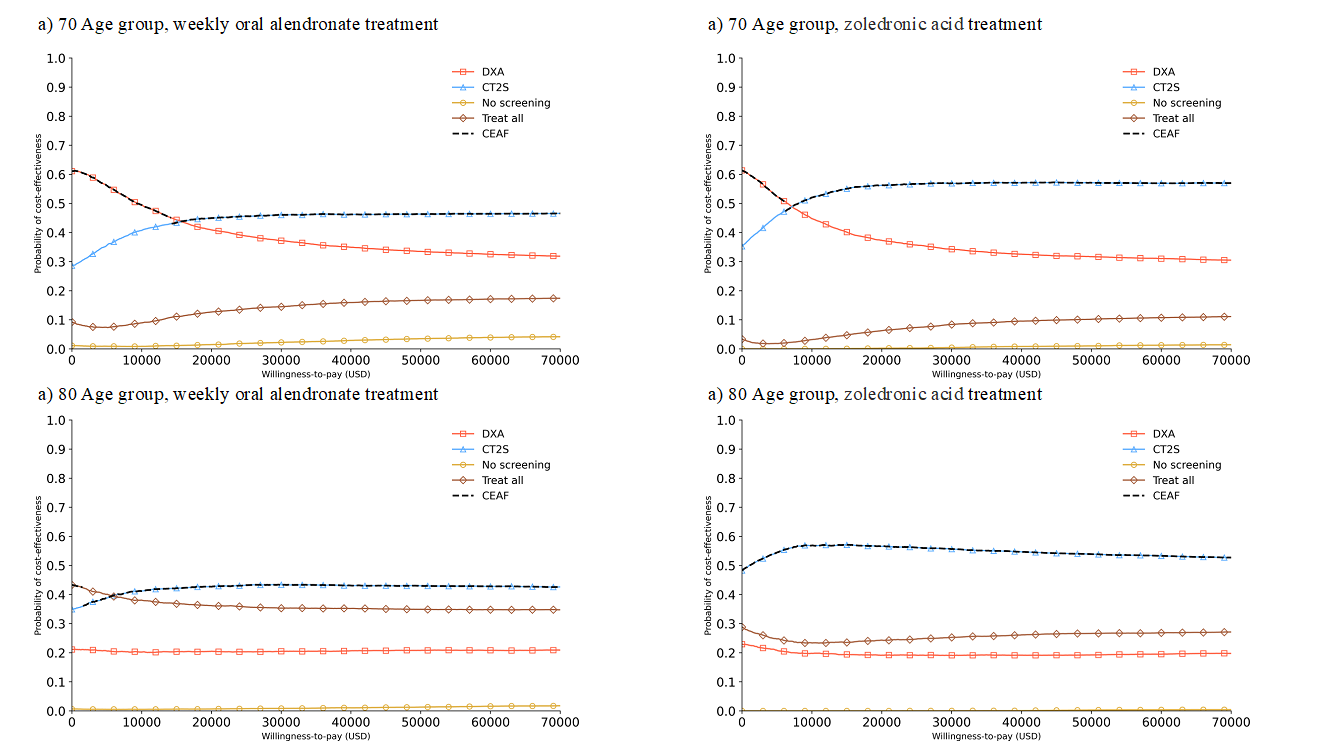
\includegraphics[width=1.0\textwidth]{4-3.png}
\caption{Cost-effectiveness acceptability curve and cost-effectiveness acceptability frontier for the 70s age group with weekly oral alendronate treatment (a) and zoledronic acid treatment (b). Cost-effectiveness acceptability curve for the 80s age group with weekly oral alendronate treatment (c) and zoledronic acid treatment (d). The other parameters are the same as the base case: screening interval = 5 years, discount rates are 4.0\% and 1.5\% for costs and effectiveness.}
\label{fig:4-3}
\end{figure}

\section{Discussion}

In this study, we applied early HTA to evaluate the cost-effectiveness of CT2S, DXA, Treat all, and No Screening strategies for osteoporosis screening and treatment in the Dutch postmenopausal women referred to FLS. These strategies were evaluated across various age groups, screening intervals, treatments, and discount rate scenarios. The aim of this research was to investigate the potential extra benefit, in terms of QALYs, and extra cost of a novel screening method, CT2S, in order to evaluate its potential economic attractiveness if adopted broadly among the FLS population in the Netherlands. To our knowledge, this was the first cost-effectiveness study for a fracture risk assessment tool using CT-based finite element model in osteoporosis screening. The findings suggest that compared to the current standard clinical approach DXA screening, CT2S has the potential to be cost-effective in women referred to Dutch FLS, especially for those within the 70s and 80s age groups. This finding of cost-effectiveness was also observed with a shorter osteoporosis screening interval of 2-years and an alternative treatment of annual zoledronic acid treatment with better adherence.

Our analysis has several strengths. The model structure allowed for realistic simulation of patients' osteoporosis case trajectories and inherently accounted for the competing risk of death. We conducted internal and external validation and showed that modelled validation output, prevalence of osteoporosis by age, lifetime risk of fracture and un-discounted, un-quality-adjusted life expectancy matched observed data quite well. In recent years, several cost-effectiveness studies have been conducted for osteoporosis screening (DXA and ultrasound) and treatment strategies \cite{4-45,4-75,4-76,4-77,4-78}. However, compared to Markov cohort models, we adopted a two-dimensional, we adopted a two-dimensional, discrete-state simulation methodology which offered two benefits. The large number of total iterations (parameter-level number multiplied by individual-level number) produced stable grand averaged lifetime costs and QALYs on which we performed our CUAs. The two-dimensional structure allowed us to assess the effect on the model output of the uncertainty surrounding input parameter point estimates as well as patient-level stochasticity expressed as cost-effectiveness acceptability curves.

To our knowledge, this was the first study in which DXA was not treated as the gold standard for osteoporosis screening (100\% accurate) since CT2S has been shown to have better discrimination between women with and without fractures. The current study addresses some of the limitations of the previous work. For example, the rescreening process was not considered in Mueller and Kingkaew's model \cite{4-75,4-77} and Li's model only considered rescreening with a 5-year screening interval \cite{4-45}. Our study considered both 5- and 2-year rescreening scenarios. In addition, Li's model only applied rescreening to people with previously negative results. However, the study by Van Gompel et al. \cite{4-19} showed approximately 60\% high-risk or osteoporotic women were re-screened within 5 years. Therefore, it was useful to simulate rescreening for all persons within FLS in the current study.

The classification accuracy of DXA and CT2S in identifying osteoporotic hip fractures has been used as the approximation of the osteoporosis screening accuracy in this study. Since osteoporotic fracture is one of the serious disease consequences of osteoporosis, and osteoporosis cannot be reversed without medication, it was reasonable to assume that the predictive accuracy cannot exceed the stratification accuracy of osteoporotic fractures for the same osteoporosis screening tool. If we treat the ``identification of osteoporosis'' was considered as finding those with a high risk of getting an osteoporotic fracture in the future, then we could treat the accuracy of the ``identification of osteoporosis'' could be treated as the predictive accuracy of getting an osteoporotic fracture in the coming 10 or 20 years. Therefore, if we use the stratification accuracy of osteoporotic fractures was used as an approximation to the identification of osteoporosis and prove it to be cost-effective, and hence elucidate that CT2S has the potential advantages in the identification of osteoporosis compared to DXA. 

The performance of CT2S, particularly its ability to accurately identify patients with osteoporosis (sensitivity), has a substantial impact on the ICER outcome, as indicated by the results of our one-way sensitivity analyses. Previous studies in the group have validated the CT2S approach using cadaver bones, which resulted in a 7-15\% standard error for failure strength and strain estimation when compared against experimental results \cite{4-6}. Part of this was attributed to the inter- and intra-observer error during the femur segmentation process, which was quantified to be within 5\%. The ARF0 (CT2S with added subject-specific fall dynamics and hip impact mechanics) was also verified with respect to all numerical approximations and achieved an overall error tolerance of 1.92 percentage points with an uncertainty of 4 percentage points due to model inputs \cite{4-6}. The CT2S input data used in this study has been carefully considered by taking results derived from the most appropriate boundary conditions to minimise potential error propagation \cite{4-7}. The range of values considered in the one-way sensitivity analysis here therefore represents the absolute worst case scenario when CT2S screening sensitivity was reduced by 20\% and 30\%, which are higher than the error range reported in previous sensitivity analyses. Future uncertainty quantification of CT2S input parameters will provide a more comprehensive understanding of its performance and enhance the robustness of cost-effectiveness analyses. Such studies could also be extended to include the application towards predicting other types of osteoporotic fractures like vertebral and wrist fractures. As early HTA analyses do not yield definitive recommendations for the development or adoption of innovations, their purpose is to contribute to ongoing discussions regarding investments, financial accountability, and reimbursement policies \cite{4-12}. In this context, our observations can contribute to the discourse surrounding the development, implementation, and reimbursement of CT2S as a potential novel osteoporosis screening tools for secondary fracture prevention.

In the current study, fixed screening intervals were adopted for both DXA and CT2S screening (5 and 2 years). In the clinical practice, the screening interval depends on the presence of risk factors and age \cite{4-79,4-80}. However, our screening interval scenarios would be expected to encompass the likely range of screening intervals that might be employed in practice. In addition, we assumed all the people within FLS were willing to cooperate and perform rescreening in fixed screening interval. This assumption is reasonable given that women chose to attend FLS at the onset, but could limit the generalisation of the CUA results to osteoporosis screening in non-FLS clinics.

The current model considered three main fractures (hip, vertebral and wrist) in our model. Other types of fractures were not considered due to the lack of relevant clinical data. This might lead to the underestimation of the potential lifetime cost savings and increase in quality-adjusted life expectancy from the prevention of other types of osteoporotic fracture. However, considering other types of fractures would serve to lower ICER values, which would strengthen the current findings of cost-effectiveness. Since the CT2S service to-date has only been used in clinical research and has not been commercialised, there was no profit margin added to the cost of CT2S. However, our estimation of CT2S screening cost is conservative and it involved setting the mean of a gamma distribution from which a cost was selected for each parameter-level iteration. These distributions covered a range of possible CTS costs. Furthermore, the automation of the CT2S image pre-processing step using open-source convolutional neural network (such as U-Net) may further reduce the cost. 

This study has several other limitations. Since the nursing home admission probability after hip fracture for Dutch population is only available for age group 80s \cite{4-69}, the admission probabilities for age groups 60s and 70s were obtained from a Norway study \cite{4-68}. In addition, while the prevalence of osteoporosis among women is nearly ten times higher than that among men in the Netherlands \cite{4-29}, it would be highly valuable to also investigate the cost-effectiveness of CT2S screening for men. Moreover, since health utilities, osteoporosis prevalence, mortality rate, and annual fracture rates for the Dutch population are not reported with confidence intervals or standard deviations, distributions were created for these parameters by assuming a standard deviation of 20\% of the mean to account for the parameter uncertainty. These data can be updated when relevant information become available in the future. The current model assumes that treatment recommendations based on DXA screening rely solely on the T-score, whereas other factors such as smoking, glucocorticoid use, and alcohol intake can be combined with the T-score in other fracture risk predictors such as the FRAX score \cite{4-81}. Unfortunately, it was not possible to include the FRAX model in this study due to a lack of required clinical data.

According to statistical data from 2020 and the report by the International Osteoporosis Foundation, there were 618 hospitals in the Netherlands in 2020, with over 50\% of these hospitals having FLS programs \cite{4-82,4-83}. However, at the national level, there are only 256 CT scanners available \cite{4-84}. This limitation may impact the future adoption of CT2S in clinical settings. Furthermore, in terms of the radiation effects of CT scan on patients, according to the study of Viceconti et al. (2018), the CT2S service recommends a whole femur CT scan protocol that results in an effective radiation dose ranging from 1.3 to 3.2 mSv for females \cite{4-4}. However, it also highlights a recent study suggests that even more aggressive reductions can be implemented without compromising the predictive accuracy \cite{4-85}. The 2018 study also demonstrates that the risk reduction in death due to complications related to hip fractures through CT2S is nearly ten times greater than the additional risk of death resulting from the additional radiation exposure for elderly women \cite{4-4}. Therefore, the radiation effects were not incorporated into the health utility of the patient in our model. Finally, this study focuses on the cost-effectiveness of CT2S osteoporosis screening in Dutch postmenopausal women and may not be directly apply to other countries and healthcare systems without recalibration of some input parameters.

In conclusion, this study demonstrated how early HTA may be applied for a potential novel osteoporosis screening tool for secondary fracture prevention in the Netherlands. The findings suggest that CT2S has the potential to be cost-effective in women referred to Dutch FLS at ages 70 and 80, compared to DXA screening, as the ICER fell below the lower bound ICER threshold in the Netherlands. The finding of cost-effectiveness was also observed with a shorter osteoporosis screening interval of 2-years and alternative treatment (annual zoledronic acid treatment) with better adherence. These findings suggest that CT2S could be used as a potential osteoporosis screening tool in the clinical setting in the Netherlands. And maybe more importantly. It raises the prospect that how high performance computing enabled simulation applications might contribute to enhanced healthcare quality and potential cost savings.







